\chapter{Semiconductors}
\label{chap:silicon}


\section{Silicon as a Semiconductor for Attosecond Spectroscopy}

\textcolor{red}{check again}

Silicon is the prototypical covalent semiconductor and, in many ways, the ``hydrogen atom'' of solid-state physics: virtually any new band-structure or many-body method is tested on crystalline Si first.\cite{Robertson1983,SemiconductorStructureOverview} 
For attosecond optical spectroscopy, silicon provides a conceptually clean but physically rich playground: it combines a well-understood covalent band structure with an indirect band gap, multiple equivalent conduction-band valleys, strong electron--phonon coupling, and a technologically important disordered/amorphous phase.

In this section we summarize the main features of the electronic structure of crystalline and disordered silicon, with emphasis on:
(i) the formation of valence and conduction bands from atomic orbitals,  
(ii) the special role of the $\Gamma$ point in the Brillouin zone, and  
(iii) how static defects and amorphous disorder modify the band structure and related properties in a way that is directly relevant to attosecond pump--probe experiments.

\subsection{Crystal structure and formation of the band structure}

Crystalline silicon adopts the diamond structure: a face-centered cubic (fcc) Bravais lattice with a two-atom basis. Each Si atom is covalently bonded to four nearest neighbours in a tetrahedral $sp^3$ configuration. The strong directional $sp^3$ bonds lead to:
\begin{itemize}
  \item a deep bonding manifold (valence bands) derived primarily from $sp^3$-like combinations of atomic $3s$ and $3p$ orbitals,
  \item a corresponding antibonding manifold (conduction bands),
  \item a band gap between predominantly bonding and antibonding states.\cite{Robertson1983}
\end{itemize}

The Brillouin zone (BZ) of the fcc lattice contains high-symmetry points $\Gamma$ (center), X (face centers), L (zone corners), and $\Delta$ lines along $\langle 100\rangle$ directions connecting $\Gamma$ and X. 
In silicon, the:
\begin{itemize}
  \item \emph{valence-band maximum} (VBM) is located at $\Gamma$,
  \item \emph{conduction-band minima} (CBM) lie at six equivalent $\Delta$ valleys, at about $0.85$ of the way from $\Gamma$ to X along each $\langle 100\rangle$ direction.\cite{WessnerSiBand,Oliphant2025}
\end{itemize}
This makes silicon an \emph{indirect} band-gap semiconductor: the minimum gap connects states with different crystal momenta.


\begin{figure}[h!] % можно [t], [b], [p], [h]
    \centering
    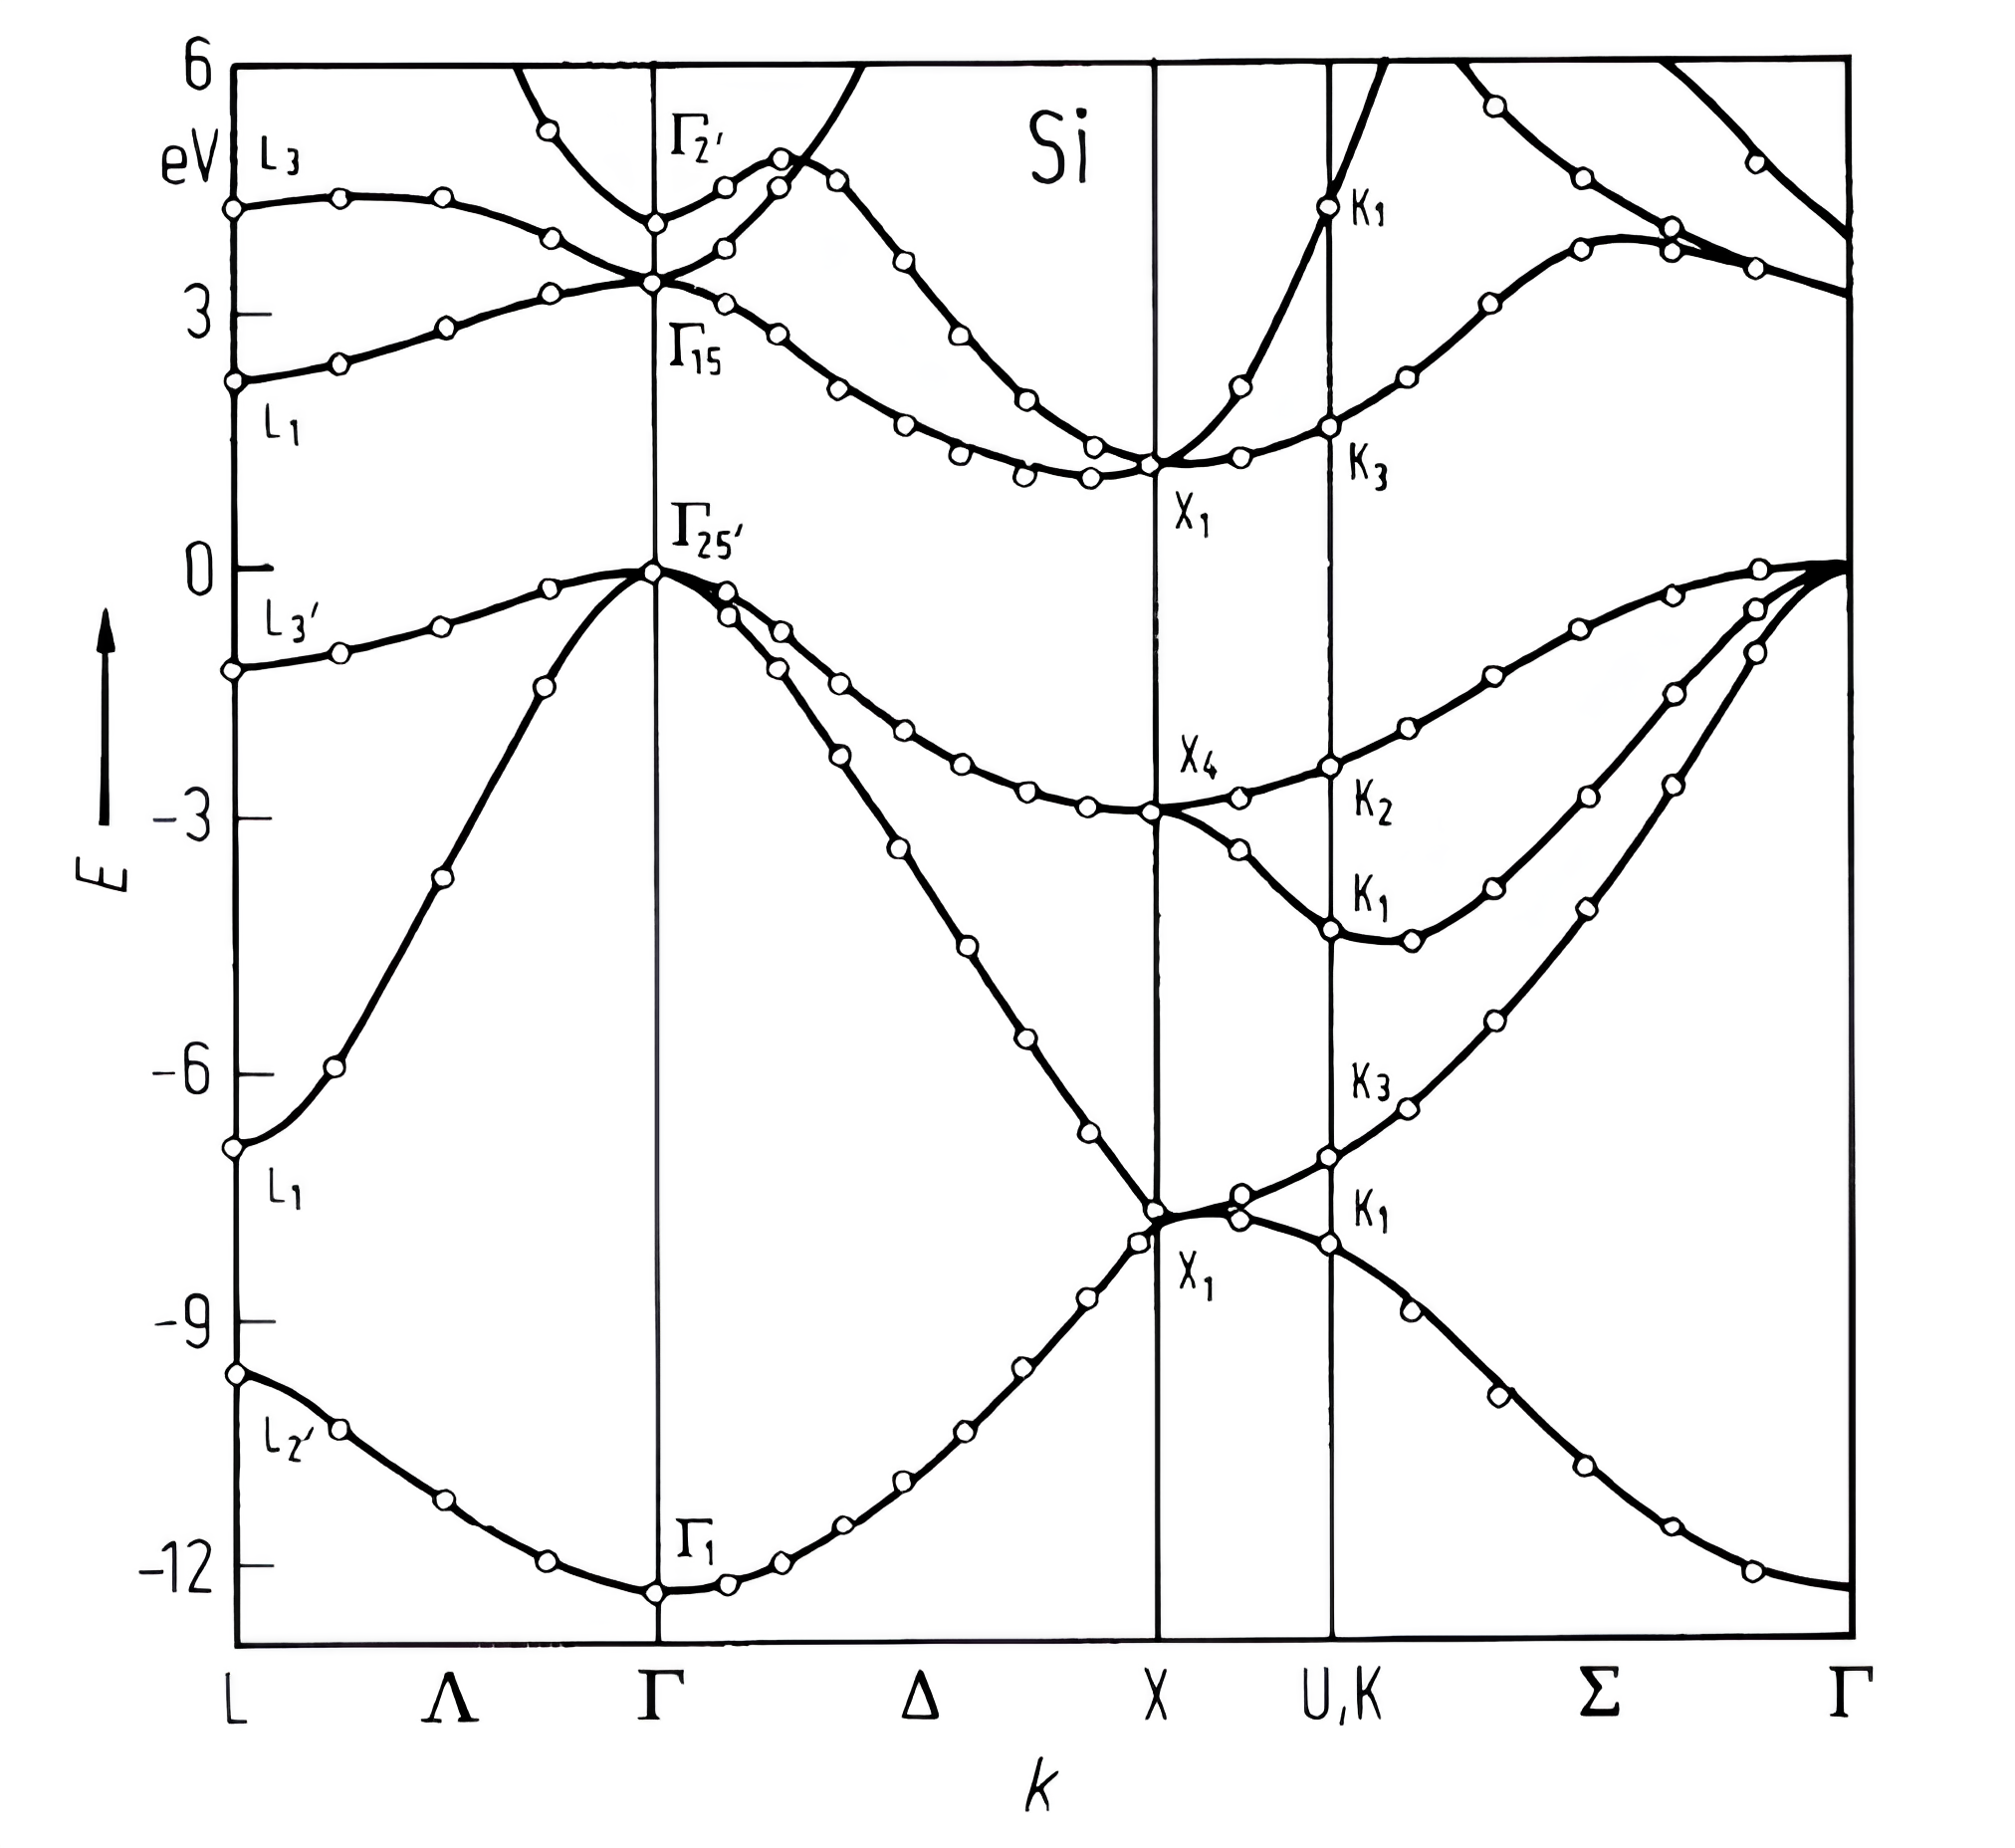
\includegraphics[width=0.6\linewidth]{figures/Si_bandstructure.png} % путь к файлу
    \caption{Band structure of silicon.}
    \label{fig:myimage}
\end{figure}

At room temperature the fundamental indirect gap is $\approx 1.12$\,eV, while the lowest direct gap at $\Gamma$ is significantly larger ($\approx 3.4$\,eV).\cite{Robertson1983,WessnerSiBand} 
Consequently, single-photon interband absorption near the band edge in bulk Si is phonon-assisted, whereas direct (vertical) optical transitions at $\Gamma$ require substantially higher photon energies.

\subsection{Electronic structure near the $\Gamma$ point}

The $\Gamma$ point ($\mathbf k=0$) is of particular interest for attosecond spectroscopy, even though Si is an indirect-gap semiconductor, for several reasons:
(i) the VBM is at $\Gamma$; 
(ii) optical matrix elements are typically largest near $\Gamma$;
(iii) the symmetry classification of states (heavy- and light-hole, split-off bands, direct $\Gamma$-conduction band) is simplest and most transparent at this point.\cite{Robertson1983,SiliconQuantumElectronics}

\subsubsection{Valence bands at $\Gamma$: heavy- and light-hole bands}

At $\Gamma$, the top of the valence band arises from three degenerate $p$-like orbitals ($p_x,p_y,p_z$) on each Si atom, combined with spin $S=1/2$. 
Spin--orbit coupling couples orbital angular momentum $L=1$ with spin, resulting in total angular momenta:
\[
J = 3/2 \quad\text{and}\quad J = 1/2.
\]
This yields:
\begin{itemize}
  \item a fourfold-degenerate $J=3/2$ manifold at the valence-band maximum, 
  \item a twofold-degenerate $J=1/2$ split-off band, lying about $44$\,meV below the VBM in Si.\cite{Robertson1983}
\end{itemize}

Within the $J=3/2$ manifold, states are usually classified as:
\begin{itemize}
  \item heavy holes (HH): $m_J = \pm 3/2$,
  \item light holes (LH): $m_J = \pm 1/2$.
\end{itemize}
At $\Gamma$ these HH and LH states are exactly degenerate in energy but differ in their effective mass along different crystallographic directions: HH bands are ``flatter'' (larger effective mass), LH bands are more dispersive (lighter mass).
For finite $\mathbf k$, HH and LH bands split and mix; however, for ultrafast optical excitation with modest $|\mathbf k|$-values, the $\Gamma$-point representation provides a good starting point.

For attosecond experiments, this structure implies that:
\begin{itemize}
  \item the initial hole population will be distributed between HH and LH branches according to the optical selection rules and polarization,
  \item the split-off band contributes only when the pump photon energy and bandwidth are sufficient to excite from that band, or when strong fields induce higher-order transitions.
\end{itemize}

\subsubsection{Conduction bands at $\Gamma$: direct gap and higher bands}

The lowest conduction-band state at $\Gamma$ is mainly $s$-like and forms the bottom of the direct gap at $\Gamma$ (often labeled $\Gamma_{15c}$ or similar in group-theoretical notation).\cite{Robertson1983}
This state is:
\begin{itemize}
  \item higher in energy than the $\Delta$-valleys that define the indirect gap,
  \item but crucial for direct optical transitions and for attosecond pump--probe experiments with sufficiently high photon energies.
\end{itemize}

Even if the pump photon energy is below the direct $\Gamma$-gap, strong-field excitation and multiphoton processes can inject carriers into $\Gamma$-like conduction states, especially for few-cycle, high-intensity pulses.
Numerical band-structure calculations and many-body simulations for Si show that the conduction-band dispersion near $\Gamma$ is relatively isotropic and parabolic at low energies, which simplifies modelling of early-time carrier dynamics in $\mathbf k$-space.\cite{WessnerSiBand,QuantumATKSi}

In the context of the present work, where the pump pulse is a few-femtosecond optical pulse and injection can be approximated as predominantly vertical (no change in $\mathbf k$), the $\Gamma$-point picture is particularly convenient:
\begin{itemize}
  \item initial excitation is treated as vertical transitions from HH/LH valence bands at $\Gamma$ to conduction states at the same $\mathbf k\simeq 0$,
  \item these $\Gamma$-conduction states then act as the ``entry point'' for subsequent (slower) scattering into the $\Delta$-valleys, which occurs on tens to hundreds of femtoseconds via electron--phonon interactions.\cite{Bernardi2014,Marini2013}
\end{itemize}
On attosecond to few-femtosecond time scales, the population remains largely in the vicinity of the initial injection region in $\mathbf k$-space, making the $\Gamma$-centric description physically meaningful.\cite{Schultze2014}

% \subsection{Relevance of the indirect gap for attosecond experiments}

% Because the fundamental gap in Si is indirect, single-photon interband transitions near the band edge must conserve both energy and momentum by involving phonons.\cite{BandStructureDirectIndirect}
% However, for attosecond and strong-field experiments:
% \begin{itemize}
%   \item the pump pulse is very short (few-fs or sub-cycle), with a correspondingly broad spectral bandwidth,
%   \item the field strengths can be high enough to induce multiphoton transitions and strong-field mixing of bands,
%   \item the XUV probe (in transient absorption) is sensitive to instantaneous changes in band occupancy and screening, rather than to the detailed phonon-assisted transition pathway.
% \end{itemize}

% Attosecond XUV spectroscopy of Si has shown that:
% \begin{itemize}
%   \item electrons injected into the conduction band by a near-IR few-cycle pump modify the XUV absorption in discrete steps synchronized with the electric-field oscillations,
%   \item the observed $\sim 450$\,as rise time of these steps sets an upper limit to the carrier-induced band-gap reduction and electron--electron scattering time in the conduction band,\cite{Schultze2014}
%   \item on this time scale, the dominant physics is coherent interband polarization and mean-field screening, which RT-TDDFT captures well.
% \end{itemize}

% Thus, for the time scales and pump parameters considered in this thesis, it is justified to treat:
% \begin{itemize}
%   \item excitation as predominantly vertical in $\mathbf k$ (``direct'' on the RT-TDDFT level),
%   \item $\Gamma$-centered states as the main injection region,
%   \item the indirectness of the gap as mainly affecting longer-time relaxation (phonon-assisted transfer to $\Delta$-valleys), which lies outside the primary attosecond window.
% \end{itemize}

% \subsection{Static defects, amorphous disorder and their impact on the band structure}

% Real silicon samples often contain static defects (vacancies, interstitials, dislocations) and, in many applications, an amorphous or nanocrystalline phase.
% Such disorder breaks translational symmetry and qualitatively modifies the electronic structure and optical response, which is central for attosecond spectroscopy of \emph{disordered} media.

\subsubsection{Point defects and extended defects in crystalline Si}

Point defects such as vacancies, interstitials and impurity atoms introduce localized states within the band gap and in the band tails:
\begin{itemize}
  \item isolated vacancies generate deep levels in the gap, 
  \item vacancy clusters and dislocation cores can create a distribution of defect states extending into the mobility gap.\cite{AtomisticBandTailSi,Drabold1999}
\end{itemize}
First-principles simulations show that such defect-induced states are strongly localized in real space and can act as trapping centers or recombination sites.\cite{AtomisticBandTailSi,AttaFynn2004}

From the band-structure point of view:
\begin{itemize}
  \item Bloch-like extended states near the valence and conduction band edges coexist with defect-localized states in the gap and tails,
  \item optical transitions involving defect states lead to additional absorption features below the crystalline band edge and to broadening of the absorption itself.
\end{itemize}
In attosecond pump--probe experiments, the presence of such localized states can:
\begin{itemize}
  \item modify the initial carrier distribution (e.g.\ by providing sub-gap absorption channels),
  \item accelerate dephasing of the macroscopic polarization due to spatial inhomogeneity,
  \item introduce additional, slower components in the transient signal related to trapping and detrapping dynamics.
\end{itemize}

\subsubsection{Amorphous silicon: band tails and mobility gap}

In amorphous silicon (a-Si), long-range translational order is absent, but the local bonding remains predominantly tetrahedral. 
This has profound consequences for the electronic structure:\cite{Robertson1983,Drabold1999}
\begin{itemize}
  \item the concept of a sharp $E(\mathbf k)$ dispersion is replaced by a density of states (DOS) with a \emph{mobility gap},
  \item the band edges are characterized by exponential band tails of localized states (Urbach tails),
  \item near the gap, states are spatially localized due to bond-angle and bond-length disorder.
\end{itemize}

Atomistic simulations and electronic-structure calculations for large models of a-Si and a-Si:H show that:\cite{Allan1998,DongDrabold1997,AttaFynn2004,Meidanshahi2019,Luo2024}
\begin{itemize}
  \item valence-band tails are mainly associated with variations in bond angles and strained bonds,
  \item conduction-band tails are more sensitive to bond-length disorder,
  \item dangling bonds (undercoordinated Si atoms) introduce mid-gap states that can dominate transport and recombination,
  \item hydrogenation (a-Si:H) passivates dangling bonds, reduces mid-gap density of states, and narrows the distribution of tail states.
\end{itemize}

Optically, amorphous silicon exhibits:
\begin{itemize}
  \item a broadened absorption edge with a characteristic Urbach energy,
  \item stronger absorption just above the mobility gap compared to crystalline Si because phonon momentum conservation is relaxed by disorder,\cite{Robertson1983,Robertson1983Review}
  \item substantial inhomogeneous broadening of interband transitions.
\end{itemize}

For attosecond spectroscopy, these features imply:
\begin{itemize}
  \item the pump predominantly excites carriers into a mixture of extended and localized tail states, rather than into a well-defined $\mathbf k$-point,
  \item the macroscopic polarization and transient absorption signals dephase more rapidly than in the crystalline case, even in the absence of explicit scattering,
  \item the concept of $\Gamma$ as a strict crystal-momentum point is no longer applicable, but the \emph{local bonding topology} inherited from crystalline Si still shapes the DOS and selection rules.
\end{itemize}
RT-TDDFT in real space is particularly well suited to this situation, since it does not rely on Bloch periodicity and naturally captures band-tail localization and static-disorder-induced dephasing.\cite{Bondi2010,Drabold1999,Dnaya2024,AttaFynn2004}

\subsubsection{Other physical properties affected by disorder}

Static disorder and amorphization also influence:
\begin{itemize}
  \item \textbf{Effective masses and mobility:} the breakdown of $\mathbf k$ as a good quantum number and the presence of localized states reduce carrier mobility; transport occurs via hopping and percolation through extended regions.\cite{Drabold1999,AttaFynn2004}
  \item \textbf{Optical constants:} refractive index $n(\omega)$ and extinction coefficient $k(\omega)$ in a-Si differ markedly from crystalline Si, especially near the band edge and in the visible range.\cite{OpticalPropsASi}
  \item \textbf{Mechanical and vibrational properties:} changes in elastic constants and vibrational density of states modify phonon spectra and thus electron--phonon coupling.\cite{Bondi2010,Zhou2023}
\end{itemize}

All of these modifications feed back into attosecond pump--probe observables:
the broadened DOS and localized tail states affect where carriers are injected and how quickly the macroscopic polarization decays; 
modified phonon spectra determine the longer-time relaxation pathways; 
and changes in $n(\omega)$ and $k(\omega)$ influence the propagation and absorption of both pump and probe pulses.

In summary, silicon as a semiconductor presents a band structure in which the $\Gamma$ point plays a central role for valence-band physics and early-time optical injection, even though the fundamental gap is indirect.
Static defects and amorphous disorder blur the sharp $\mathbf k$-space picture and generate band tails and localized gap states, which are crucial for interpreting attosecond optical spectroscopy of disordered media.
RT-TDDFT in real space provides a natural framework to treat both the crystalline reference and its disordered realizations on equal microscopic footing.

